\section{Extended Kalman Filter}

Consider a state-space model with nonlinear dynamics:
\[\mathcal{S}:\begin{cases}
    x(t+1)=f(x(t),u(t))+v_1(t) \\
    y(t)=h(x(t))+v_2(t)
\end{cases}\]
Here, $f(\cdot)$ and $h(\cdot)$ are nonlinear functions of class $C^1$ or higher.

The Extended Kalman Filter is a variant of the Kalman Filter designed to handle nonlinear dynamics and measurements. 
It approximates the nonlinear system by linearizing it at each time step around the current estimate of the state.
To illustrate the idea, let's consider the following block diagram of the Extended Kalman Filter:
\begin{figure}[H]
    \centering
    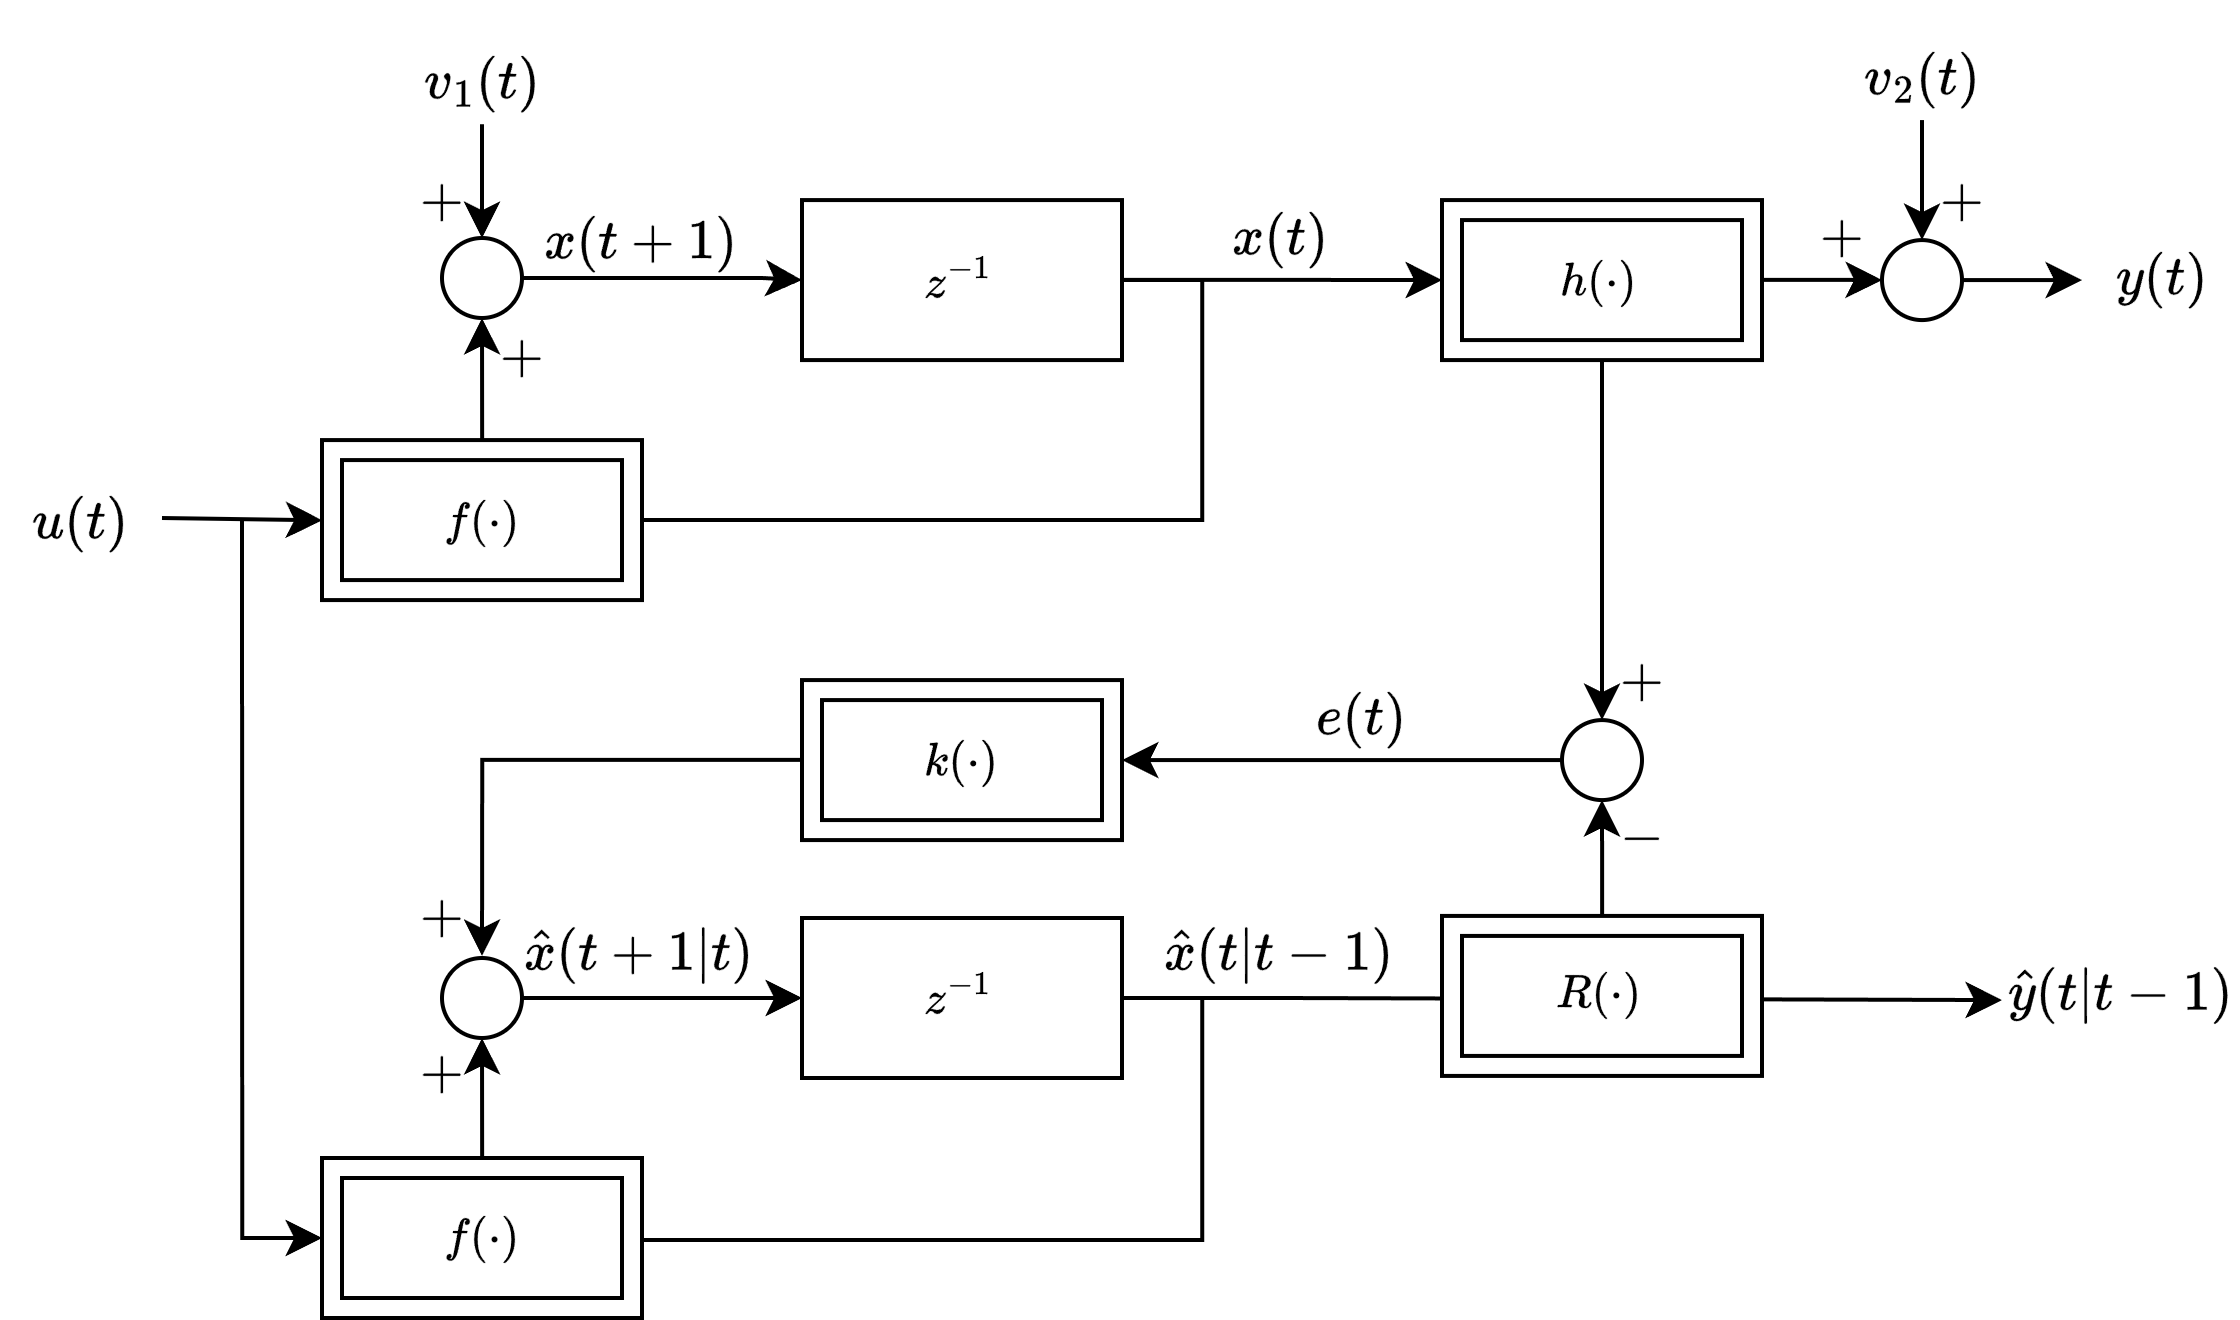
\includegraphics[width=0.75\linewidth]{images/ekf.png}
    \caption{Extended Kalman Filter block scheme}
\end{figure}
To establish the feedback correction gain, we have two distinct options:
\begin{enumerate}
    \item The gain is structured as a nonlinear function, denoted as $K(\cdot)$, yielding an output of $K(e(t))$. 
    \item Alternatively, the gain takes the form of a linear time-variant block akin to the Kalman Filter, producing an output of $K(t)e(t)$. 
\end{enumerate}
The Extended Kalman Filter embraces the latter approach, albeit less intuitive, it proves more efficacious by leveraging established theory from traditional Kalman Filters.

To easily compute the gain $K(t)$ using the Kalman Filter formula, we utilize the following equations:
\[\begin{cases}
    K(t)=\left(FP(t)H^T+V_{12}\right)\left(FP(t)H^T+V_2\right)^{-1} \\
    P(t+1)=\left(FP(T)F^T+V_1\right)-\left(FP(t)H^T+V_{12}\right)\left(HP(t)H^T+V_{2}\right)^{-1}\left(FP(t)H^T+V_{12}\right)^T
\end{cases}\]
To implement this formula, we require a method for computing $F(t)$ and $H(t)$ at each sampling instant:
\[F(t)=\dfrac{\partial f(x(t),u(t))}{\partial x(t)} \qquad H(t)=\dfrac{\partial h(x(t))}{\partial x(t)}\]
These derivatives are assessed at $x(t)=\hat{x}(t|t-1)$. 
Hence, $F(t)$ and $H(t)$ become time-varying matrices acquired through the local linearization of the nonlinear system around the predicted state vector from the preceding step.

In practice, the Extended Kalman Filter aims to convert a nonlinear, time-invariant system into a linear, time-varying system. 
Subsequently, it employs the Kalman Filter methodology on this transformed linear system.

The general procedure for the Extended Kalman Filter at the current time $t$ is outlined as follows:
\begin{enumerate}
    \item Utilize the most recent state prediction, denoted as $\hat{x}(t|t-1)$. 
    \item Employ $\hat{x}(t|t-1)$ to compute $F(t)$ and $H(t)$. 
    \item Calculate $K(t)$  and update the Differential Riccati Equation, thereby determining $P(t+1)$. 
    \item Compute $\hat{x}(t+1|t)$ for the subsequent iteration.
\end{enumerate}
This iterative procedure must be repeated for each sampling instant. 

\paragraph*{Remarks}
The Extended Kalman Filter stands out for its efficacy in handling nonlinear systems. 
However, due to its inherent nature as a nonlinear, time-variant system, it lacks a steady-state solution. 
Consequently, several implications arise:
\begin{itemize}
    \item Achieving asymptotic stability is challenging or infeasible, necessitating extensive empirical validation.
    \item Computational burden: with each sampling instance, recalculations of $F(t)$, $H(t)$, $P(t)$, and $K(t)$ are required.
\end{itemize}
While the Extended Kalman Filter finds widespread application, it encounters limitations in scenarios involving safety critical systems and applications, and mission critical systems and applications. 
\begin{example}
    Let's examine the dynamics of the following system:
    \begin{figure}[H]
        \centering
        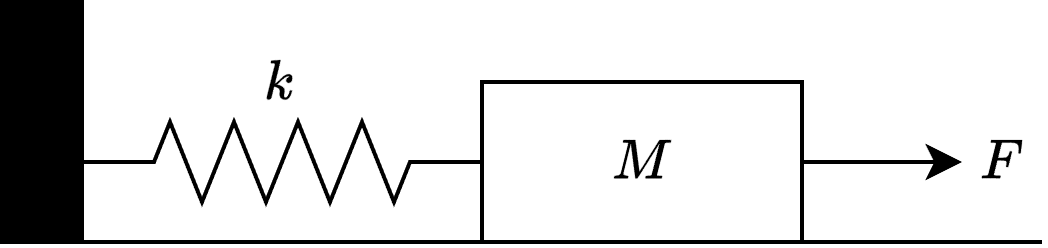
\includegraphics[width=0.4\linewidth]{images/example.png}
    \end{figure}
    Here, an object slides on a horizontal plane, connected to a wall by a spring and experiencing sliding friction.
    The input to the system is the applied force $F(t)$, while the output, measured by a sensor, is the object's position $x(t)$. 
    Our objective is to estimate the object's velocity $\dot{x}(t)$. 

    The solution to this problem involves the following steps:
    \begin{enumerate}
        \item To build the system model, we start with a white box approach in the continuous-time domain. 
            According to the second law of Newton, we have:
            \[\ddot{x}(t)M=-kx(t)-c\dot{x}(t)+F(t)\]
            Here, $kx(t)$ represents the elastic force, and $c\dot{x}(t)$ is the friction force.
            This equation is second-order linear, allowing us to describe it with two state variables.
            Given that it's a mechanical system, the natural states are the position $x(t)$ and velocity $\dot{x}(t)$:
            \[\begin{bmatrix} x_1(t)=x(t) \\ x_2(t)=\dot{x}(t) \end{bmatrix}\]
            We can transform the second-order differential equation into a system of two first-order differential equations:
            \[\begin{cases}
                \dot{x}_1(t)=x_2(t) \\
                \dot{x}_2(t)=-\frac{k}{M}x_1(t)-\frac{c}{M}x_2(t)+\frac{1}{M}F(t) \\
                y(t)=x_1(t)
            \end{cases}\]
            This formulation represents the state-space representation in continuous time.
        \item Moving from continuous time to discrete time involves discretizing the differential equations. 
            One commonly used method is the Euler forward discretization, denoted as $n$: 
            \[\dot{x}(t)\approx\dfrac{x(t+1)-x(t)}{\Delta}\]
            Here, $\Delta$ represents the sampling time.
            Applying this approximation, we get: 
            \[\begin{cases}
                \frac{x_1(t+1)-x_1(t)}{\Delta}=x_2(t) \\
                \frac{x_2(t+1)-x_2(t)}{\Delta}=-\frac{k}{M}x_1(t)-\frac{c}{M}x_2(t)+\frac{1}{M}F(t) \\
                y(t)=x_1(t)
            \end{cases}\]
            Rearranging this system into standard state-space representation form, we obtain:
            \[\begin{cases}
                x_1(t+1)=\Delta x_2(t) \\
                x_2(t+1)=-\frac{k\Delta}{M}x_1(t)-\left(1-\frac{c\Delta}{M}\right)x_2(t)+\frac{\Delta}{M}F(t) \\
                y(t)=x_1(t)
            \end{cases}\]
        \item Adding noise terms, the system equations become:
            \[\begin{cases}
                x_1(t+1)=\Delta x_2(t)+v_{11}(t) \\
                x_2(t+1)=-\frac{k\Delta}{M}x_1(t)-\left(1-\frac{c\Delta}{M}\right)x_2(t)+\frac{\Delta}{M}F(t)+v_{12}(t) \\
                y(t)=x_1(t)+v_2(t)
            \end{cases}\]
            Here, the noise vectors are defined as:
            \[v_1(t)=\begin{bmatrix} v_{11}(t) \\ v_{12}(t) \end{bmatrix} \sim WN(0,V_1) \quad v_2(t)\sim WN(0,V_2)\]
            The noise $V_2$ is determined using sensor data sheets. 
            However, noise $V_1$ is typically more intricate and often simplified as:
            \[V_1=\begin{bmatrix}
                \lambda_1^2 & 0 \\
                0 & \lambda_2^2 
            \end{bmatrix}\]
            Here, $\lambda_1^2$ and $\lambda_2^2$ are empirically adjusted.
    \end{enumerate}
\end{example}
The exploration of meta-parameters within the Kalman Filter structure represents a new avenue in machine learning.